\documentclass{beamer}

\newcommand{\course}{CS 1331 Introduction to Object Oriented Programming}
\newcommand{\lesson}{Searching and Sorting}
\newcommand{\code}{http://www.cc.gatech.edu/~simpkins/teaching/gatech/cs1331/code}

\author[Chris Simpkins] 
{Christopher Simpkins \\\texttt{chris.simpkins@gatech.edu}}
\institute[Georgia Tech] % (optional, but mostly needed)

\date[CS 1331]{}


\newcommand{\course}{Introduction to Object-Oriented Programming}
\subject{\course}
\title[\lesson]{\course}
\subtitle{\lesson}

\author[CS 1331]
{Christopher Simpkins \\\texttt{chris.simpkins@gatech.edu}}
\institute[Georgia Tech]

\date[]{}

\newcommand{\link}[2]{\href{#1}{\textcolor{blue}{\underline{#2}}}}
\newcommand{\code}{http://www.cc.gatech.edu/~simpkins/teaching/gatech/cs1331/code}

\usepackage{colortbl}

% If you have a file called "university-logo-filename.xxx", where xxx
% is a graphic format that can be processed by latex or pdflatex,
% resp., then you can add a logo as follows:

% \pgfdeclareimage[width=0.6in]{coc-logo}{cc_2012_logo}
% \logo{\pgfuseimage{coc-logo}}

\mode<presentation>
{
  \usetheme{Berlin}
  \useoutertheme{infolines}

  % or ...

 \setbeamercovered{transparent}
  % or whatever (possibly just delete it)
}

\usepackage{tikz}
% Optional PGF libraries
\usepackage{pgflibraryarrows}
\usepackage{pgflibrarysnakes}
\usepackage{pgfplots}
\usepackage{fancybox}
\usepackage{listings}
\usepackage[abbr]{harvard}
\usepackage{hyperref}
\hypersetup{colorlinks=true,urlcolor=blue}
\usepackage[english]{babel}
% or whatever

\usepackage[latin1]{inputenc}
% or whatever

\usepackage{times}
\usepackage[T1]{fontenc}
% Or whatever. Note that the encoding and the font should match. If T1
% does not look nice, try deleting the line with the fontenc.


\usepackage{listings}

% "define" Scala
\lstdefinelanguage{scala}{
  morekeywords={abstract,case,catch,class,def,%
    do,else,extends,false,final,finally,%
    for,if,implicit,import,match,mixin,%
    new,null,object,override,package,%
    private,protected,requires,return,sealed,%
    super,this,throw,trait,true,try,%
    type,val,var,while,with,yield},
  otherkeywords={=>,<-,<\%,<:,>:,\#,@},
  sensitive=true,
  morecomment=[l]{//},
  morecomment=[n]{/*}{*/},
  morestring=[b]",
  morestring=[b]',
  morestring=[b]""",
}

\usepackage{color}
\definecolor{dkgreen}{rgb}{0,0.6,0}
\definecolor{gray}{rgb}{0.5,0.5,0.5}
\definecolor{mauve}{rgb}{0.58,0,0.82}

% Default settings for code listings
\lstset{frame=tb,
  language=scala,
  aboveskip=2mm,
  belowskip=2mm,
  showstringspaces=false,
  columns=flexible,
  basicstyle={\scriptsize\ttfamily},
  numbers=none,
  numberstyle=\tiny\color{gray},
  keywordstyle=\color{blue},
  commentstyle=\color{dkgreen},
  stringstyle=\color{mauve},
  frame=single,
  breaklines=true,
  breakatwhitespace=true,
  keepspaces=true
  %tabsize=3
}


% If you wish to uncover everything in a step-wise fashion, uncomment
% the following command: 

% \beamerdefaultoverlayspecification{<+->}


\begin{document}

\begin{frame}{Searching and Sorting}
%  \titlepage
\vspace{-.1in}
  \begin{center} 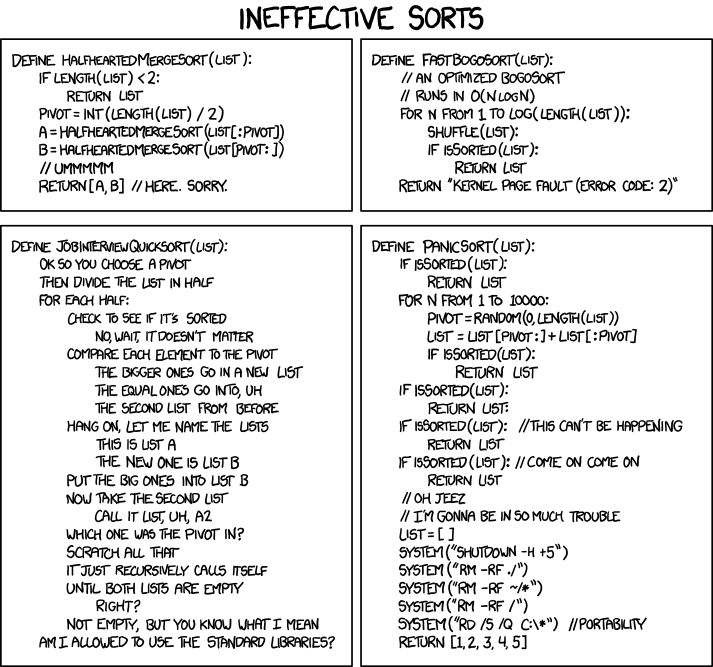
\includegraphics[height=2.9in]{ineffective_sorts.png}\footnote{\link{http://xkcd.com/1185/}{http://xkcd.com/1185/}}
  \end{center}
\end{frame}



%------------------------------------------------------------------------
\begin{frame}[fragile]{The Search Problem}


\begin{lstlisting}[language=Java]

\end{lstlisting}

\begin{itemize}
\item Input: A sequence of $n$ elements $A = <a_1, a_2, ..., a_n>$ and a value $v$
\item Output: An index $i$ such that $v = A[i]$ or a special value such as -1 or $nil$ if $v$ does not appear in $A$.
\end{itemize}


\end{frame}
%------------------------------------------------------------------------


%------------------------------------------------------------------------
\begin{frame}[fragile]{Linear Search}


Linear search is required when
\begin{itemize}
\item with an unsorted list, or
\item a linked list that does not provide indexed access to any element.
\end{itemize}


\end{frame}
%------------------------------------------------------------------------


%------------------------------------------------------------------------
\begin{frame}[fragile]{Binary Search}


If your list is sorted and you can access elements by index, you can use a binary search.
\begin{itemize}
\item
\end{itemize}

\begin{lstlisting}[language=Java]

\end{lstlisting}


\end{frame}
%------------------------------------------------------------------------


%------------------------------------------------------------------------
\begin{frame}[fragile]{Binary Search and Binary Trees}


\begin{lstlisting}[language=Java]

\end{lstlisting}

\begin{itemize}
\item
\end{itemize}


\end{frame}
%------------------------------------------------------------------------


%------------------------------------------------------------------------
\begin{frame}[fragile]{The Sorting Problem}


\begin{lstlisting}[language=Java]

\end{lstlisting}

\begin{itemize}
\item
\end{itemize}


\end{frame}
%------------------------------------------------------------------------


%------------------------------------------------------------------------
\begin{frame}[fragile]{Insertion Sort}


The insertion sort algorithm in pseudocode (from CLRS Chapter 2):
\vspace{-.05in}
\begin{lstlisting}[]
1 for j = 2 to A.length // A[1 .. A.length] is an array
2     key = A[j]
3     // Insert A[j] into the sorted sequence A[i .. j - 1].
4     i = j - 1
5     while i > 0 and A[i] > key
6         A[i + 1] = A[i]
7         i = i - 1
8    A[i + 1] = key
\end{lstlisting}

Insertion sort implemented in Java:
\vspace{-.05in}
\begin{lstlisting}[language=Java]
for (int j = 1; j < a.length; ++j) {
    int key = a[j];
    int i = j - 1;
    while(i >= 0 \&\& a[i] > key) {
        a[i + 1] = a[i];
        i = i - 1;
    }
    a[i + 1] = key;
}
\end{lstlisting}

\end{frame}
%------------------------------------------------------------------------


%------------------------------------------------------------------------
\begin{frame}[fragile]{}


\begin{lstlisting}[language=Java]

\end{lstlisting}

\begin{itemize}
\item
\end{itemize}


\end{frame}
%------------------------------------------------------------------------


%------------------------------------------------------------------------
\begin{frame}[fragile]{}


\begin{lstlisting}[language=Java]

\end{lstlisting}

\begin{itemize}
\item
\end{itemize}


\end{frame}
%------------------------------------------------------------------------


%------------------------------------------------------------------------
\begin{frame}[fragile]{}


\begin{lstlisting}[language=Java]

\end{lstlisting}

\begin{itemize}
\item
\end{itemize}


\end{frame}
%------------------------------------------------------------------------

% %------------------------------------------------------------------------
% \begin{frame}[fragile]{}


% \begin{lstlisting}[language=Java]

% \end{lstlisting}

% \begin{itemize}
% \item
% \end{itemize}


% \end{frame}
% %------------------------------------------------------------------------



\end{document}
